\chapter{Gravitational physics}\label{gravphys}

The following section reviews key concepts of Newton’s theory of gravitation to motivate differences with their respective relativistic versions later in the chapter. Concepts such as multipole moments and self-gravitating bodies in hydrostatic equilibrium in the Newtonian limit will be presented in detail as they play a fundamental role in generating gravitational waves and state-of-the-art numerical relativity simulations of compact binary mergers. 


\section{Newtonian gravity}

It is surprising how well Newtonian gravity reproduces the effects of systems in the presence of weak gravitational fields. For centuries astronomers could make predictions using Newton's theory and confirm its versatility in systems such as main sequence stars, galaxies, the Earth-Moon system, and planets of the solar system (not without problems). For this reason, it is taken as a reference for more modern theories of gravity, which by convention are asked to reproduce its effects in the slow motion approximation,i.e., $\frac{||\vec{v}||}{c} << 1$ and weak field limit $\frac{GM}{c^2 R} <<1$. It is important to emphasize that it is an incomplete theory. Although it works well in the examples mentioned, it cannot reproduce phenomena such as gravitational lensing, gravitational redshift, and gravitational waves.


The following sections will present the fundamentals of newton's theory of gravitation to speak of generalized mass distributions and their gravitational fields motivated by the descriptions made in books by Shapiro\cite{Shapiro:1983du} and Poisson \cite{poisson_will_2014}.

Let us begin by introducing the field equations of Newtonian gravity. Although Newton's work in gravitation is better known by the inverse square law, the description of Newtonian gravity as a field theory via Poisson's equation is more modern. It allows us to see its simplicity and establish its differences from Einstein's field equations. Poisson's equation for gravitation and its solution in terms of green's functions can be written down as 

\begin{equation}\label{poisson}
\nabla^2 \phi = -4\pi G \rho(t, \vec{x}).
\end{equation}

\begin{equation}\label{phi}
\phi(t, \vec{x}) = -4\pi G \left( \frac{1}{4\pi} \int_{V} \frac{\rho(t, \vec{x}')}{|| \vec{x}-\vec{x}' ||} d^3x'\right).
\end{equation}

Where G is the gravitational constant. From which one can naturally define the active gravitational mass as the flux of the force field $\vec{g}=-\vec{\nabla} \phi(t, \vec{x}')$ and its flux through the surface $\partial V$ 

\begin{equation}
dm(t, \vec{x}) = \frac{1}{4\pi G} \cdot \vec{\nabla}(\vec{\nabla}\phi) dV,
\end{equation}

\begin{equation}
m(t, \vec{x}) = -\frac{1}{4\pi G}\int_{V} \vec{\nabla} \cdot (\vec{\nabla} \phi(t, \vec{x}')) d^3 x' ,
\end{equation}

\begin{equation}\label{active mass}
m(t, \vec{x}) = \frac{1}{4\pi G}\int_{\partial V}  \vec{g}\cdot \hat{n}  \;\; d^2 x'.
\end{equation}


Where $\hat{n}$ represents the unit normal vector field to the surface $\partial V$. Solutions to equation \ref{phi}, together with Newton's second law, and an equation of state, allow us to compute interesting physical observables like the orbits of bodies in the presence of the field $\phi$, the internal structure of self-gravitating objects and their binding energy.


In general, solutions to equation \ref{poisson} can be computed using analytical methods as in electromagnetism(see \cite{Jackson:1998nia}), numerical methods, or the multipole expansion (see for example \cite{Thorne:1980ru}). The latter method is a powerful tool to perform approximate analytical calculations on bodies with complicated geometries and is described in detail in the following subsection. It has been widely used in experiments on the solar system and to measure earth's surface potential\cite{GOCE, GRACE}. 




\subsection{The multipole expansion}

Series expansions are a systematic tool for working with gravitational fields produced by complicated mass distributions. Analytical calculations and gravitational physics experiments  in Earth's orbit often use spherical coordinates to decompose the function $\frac{\alpha}{||\vec{x}-\vec{x'}||}$ in terms of its spherical harmonics \cite{Muller,kaula1966theory,Stirling:2017ybn}. However, the derivation of the multipole expansion will be presented below in Cartesian coordinates to match the conventions of the gravitational wave section in the books by Hartle \cite{Hartle:2021pel} and Creighton \cite{Creighton:2011zz}.

Let us begin by writing down the Taylor expansion of a scalar field $f$


\begin{equation}\label{tay1}
f(x') = f(x')\Biggr|_{\vec{x'_0}} + ((x-x'_0)\cdot \nabla) f(x)\Biggr|_{\vec{x'_0}} + \frac{1}{2!} ((x-x'_0)\cdot \nabla)((x-x'_0)\cdot \nabla) f(x)\Biggr|_{\vec{x'_0}} + ...
\end{equation}

Which can also be expressed by components using a Cartesian orthonormal basis $e_b:= {\hat{i}, \hat{j},\hat{k}}$ . Such that the differential operator $\nabla$ becomes $\frac{\partial}{\partial x^a} \theta^a$ and the vector $(x-x'_0)$ can be rewritten as $(x - x'_0)^b e_b$. Where $\theta^a$ is the dual basis given by 

$$\theta^a e_b= \delta^a_b$$

Then, equation\ref{tay1} becomes 

%\begin{equation}
\begin{multline}
f(x'^a) = f\Biggr|_{\vec{x'_0}} + \left( \frac{\partial f}{\partial x'^a} \theta^a \right)\Biggr|_{\vec{x'_0}} (x' - x'_0)^b e_b \\ + \frac{1}{2!} \left( \frac{\partial^2 f}{\partial x'^a \partial x'^b} \theta^a \otimes \theta^b \right)\Biggr|_{\vec{x'_0}} (x' - x'_0)^c e_c (x' - x'_0)^d e_d + ...\;\; ,
\end{multline}
%\end{equation}

\begin{equation}\label{tay.exp}
f(x'^a) = f\Biggr|_{\vec{x'_0}} + \left( \frac{\partial f}{\partial x'^a} \right)\Biggr|_{\vec{x'_0}} (x' - x'_0)^b \delta^a_b + \frac{1}{2!} \left( \frac{\partial^2 f}{\partial x'^a \partial x'^b}  \right)\Biggr|_{\vec{x'_0}} (x' - x'_0)^c  (x' - x'_0)^d \delta^a_d \delta^b_d +   ... \;\; ,
\end{equation}

%\begin{multline}
%\left( \frac{1}{|| \vec{x} - \vec{x}'||} \right) = \left( \frac{1}{|| \vec{x} - \vec{x}'||} \right)\Biggr|_{\vec{x'_0}} + \left( \frac{\partial \left( \frac{1}{|| \vec{x} - \vec{x}'||} \right)}{\partial x'^a} \right)\Biggr|_{\vec{x'_0}} (x' - x'_0)^b \delta^a_b \\+ \frac{1}{2!} \left( \frac{\partial^2 \left( \frac{1}{|| \vec{x} - \vec{x}'||} \right)}{\partial x'^a \partial x'^b}  \right)\Biggr|_{\vec{x'_0}} (x' - x'_0)^c  (x' - x'_0)^d \delta^a_d \delta^b_d + ... \;\;.
%\end{multline}


Now, let's apply the expansion \ref{tay.exp} to the function $\frac{1}{||\vec{x}-\vec{x'}||}$. To do this, we first write its denominator in components and calculate its first and second derivatives:

$$ \frac{1}{|\vec{x}-\vec{x'}|} \rightarrow \frac{1}{(\delta_{ab} (x- x')^a (x- x')^b)^\frac{1}{2}}$$

\begin{equation}\label{first der.}
\frac{\partial}{\partial x'^a}(\delta_{cd} (x- x')^c (x- x')^d)^{-\frac{1}{2}} = \frac{(x_a - x'_a)}{(\delta_{cd} (x- x')^c (x- x')^d)^{\frac{3}{2}}} \;\; ,
\end{equation}

\begin{multline}\label{second der.}
\frac{\partial^2}{\partial x'^a \partial x'^b}(\delta_{cd} (x- x')^c (x- x')^d)^{-\frac{1}{2}} = \frac{-\delta_{ab}}{(\delta_{cd} (x- x')^c (x- x')^d)^{\frac{3}{2}}}\\ +\frac{3(x_a - x'_a)(x_b - x'_b)}{ (\delta_{cd} (x- x')^d (x- x')^d)^{\frac{5}{2}} } \;\; .
\end{multline}


Inserting  \ref{first der.} and \ref{second der.} into the first two terms of the expansion \ref{tay.exp}, and taking $\vec{x}_0 = \vec{0}$, the expansion becomes: 

\begin{equation}
\left( \frac{1}{|| \vec{x} - \vec{x}'||} \right) = \left( \frac{1}{|| \vec{x}||} \right) + \frac{x_a x'^b \delta^a_b}{||\vec{x}||^3} + \frac{1}{2!} \left(\frac{-\delta_{ab}}{||\vec{x}||^3} + \frac{3 x_a x_b}{||\vec{x}||^5}  \right) x'^c x'^d \delta^a_c \delta^b_d +  ... \;\; ,
\end{equation}


\begin{equation}
\left( \frac{1}{|| \vec{x} - \vec{x}'||} \right)(x'^a) = \left( \frac{1}{r} \right) + \frac{n_a x'^a}{r^2} + \\ \frac{1}{2!} \left(\frac{ 3 n_a n_b -\delta_{ab}}{r^3}  \right) x'^a x'^b + O(r^{-4})\;\; .
\end{equation}


Where $r = ||\vec{x}||$ and $n_a = \frac{x_a}{r}$. We truncate the series on the third term so that the gravitational potential \ref{phi} 

\begin{equation}\label{multipole0}
\phi(t, \vec{x}) = -G \int_{\Omega} d^3x' \rho(t, \vec{x}) \left[ \frac{1}{r} + \frac{n_a x'^a}{r^2} + \frac{1}{2} \left( \frac{ 3 n_a n_b -\delta_{ab} }{r^3}  \right) x'^a x'^b \right]
\end{equation}


\begin{equation}\label{multipole1}
\phi(t, \vec{x}) = -G \left[ \frac{\mathcal{M}}{r} + \frac{n_a \mathcal{D}^a}{r^2} + \frac{1}{2} \frac{ \left( 3 n_a n_b -\delta_{ab} \right) \mathcal{Q}^{ab} }{r^3} \right]
\end{equation}

$\mathcal{M}$, $\mathcal{D}^a$ and $\mathcal{Q}^{ab}$ are called monopole, dipole and quadrupole moments respectively

\begin{equation}
\mathcal{M} := \int_{\Omega} d^3x' \;\; \rho(t, \vec{x}'),
\end{equation}


\begin{equation}
\mathcal{D}^a := \int_{\Omega} d^3x' \;\; x'^a \rho(t, \vec{x}'),
\end{equation}


\begin{equation}\label{quadrupole}
\mathcal{Q}^{ab} := \int_{\Omega} d^3 x' \;\;x'^a x'^b \rho(t, \vec{x}').
\end{equation}


%\textit{Remark}: one can always rewrite the third term by adding a traceless extra term, for example, $-r^2 \delta^{ab}$ 
%
%$$
%\left( n_a n_b - \frac{1}{3} \delta_{ab}\right) \left( 3 x'^a x'^b - r^2\delta^{ab} \right) = \left( n_a n_b - \frac{1}{3} \delta_{ab} \right) 3 x'^a x'^b - r^2 \delta^{ab} (n_a n_b - \frac{1}{3} \delta_{ab})
%$$
%
%$$
%\left( n_a n_b - \frac{1}{3} \delta_{ab}\right) \left( 3 x'^a x'^b - r^2\delta^{ab} \right) = \left( n_a n_b - \frac{1}{3} \delta_{ab}\right) 3 x'^a x'^b - \cancel{r^2 (1-1)}
%$$
%
%So that the gravitational potential can be separated into monopole, dipole, and quadrupole moment contributions 
%$$
%\phi(t, \vec{x}) = -G \int_{\Omega} d^3x' \rho(t, \vec{x}) \left[ \frac{1}{r} + \frac{n_a x'^a}{r^2} + \frac{1}{2} \left( \frac{ \left( n_a n_b - \frac{1}{3} \delta_{ab}\right) \left( 3 x'^a x'^b - r^2\delta^{ab} \right) }{r^3}  \right) \right]
%$$
%
%$$
%\phi(t, \vec{x}) = -G \int_{\Omega} d^3x' \rho(t, \vec{x}) \left[ \frac{1}{r} + \frac{n_a x'^a}{r^2} + \frac{1}{2} \frac{ \left( n_a n_b - \frac{1}{3} \delta_{ab}\right) \left( 3 x'^a x'^b - r^2\delta^{ab} \right) }{r^3} \right]
%$$
%
%\begin{equation}\label{multipole1}
%\phi(t, \vec{x}) = -G \left[ \frac{\mathcal{M}}{r} + \frac{n_a \mathcal{D}^a}{r^2} + \frac{1}{2} \frac{ \left( n_a n_b - \frac{1}{3} \delta_{ab}\right) \mathcal{Q}^{ab} }{r^3} \right]
%\end{equation}
%
%
%$$
%\mathcal{M} := \int_{\Omega} d^3x' \;\; \rho(t, \vec{x}')
%$$
%
%$$
%\mathcal{D}^a := \int_{\Omega} d^3x' \;\; x'^a \rho(t, \vec{x}')
%$$
%
%$$
%\mathcal{Q}^{ab} := \int_{\Omega} d^3 x' \;\;x'^a x'^b \rho(t, \vec{x}) =  \int_{\Omega} d^3 x' \left( 3 x'^a x'^b - r^2\delta^{ab} \right) \rho(t, \vec{x}')
%$$

The quadrupole moment gets to be an extremely relevant quantity when studying extended bodies and tidal interactions. Given two neighboring particles, their separation vector $\vec{X}$ with components $X^i = \{X^x, X^y, X^z \} $ in presence of an external gravitational field $\phi_{ext}$, evolves according to 


\begin{equation}\label{tidal0}
\frac{d^2 X^{i}}{dt^2} = - \mathcal{E}_{ij} X^{j}
\end{equation} 

Where $\mathcal{E}_{ij}$ is called the quadrupolar tidal field, and it is given by the second derivatives of the field 

\begin{equation}
\mathcal{E}_{ij} = \frac{\partial^2 \phi_{ext}}{\partial x_i \partial x_j}
\end{equation}

Which for the case of linear tides(see \cite{poisson_will_2014, Hinderer:2007mb}) its directly proportional to the induced quadrupole moment by $\phi_{ext}$

\begin{equation}
Q_{ij} = \Lambda \mathcal{E}_{ij} = \frac{2k_2 R^5}{3G} \mathcal{E}_{ij}
\end{equation}

Where the constant of proportionality $\Lambda$ is called tidal deformability, which is related to the $l=2$ tidal love number $k_2$

\begin{equation}\label{Tid}
\Lambda = \frac{2}{3}\frac{k_2 R^5}{G}
\end{equation}

Equation \ref{quadrupole} contributes to the generation of ocean tides on Earth in the presence of the Moon's gravitational field \cite{Hartle:2021pel}. In addition, measurements of the Sun's quadrupole moment have been crucial in helioseismology and solar system physics. It also plays a fundamental role in generating gravitational waves in general relativity. As it will be shown later, only sources with a time-varying quadrupole momentum emit gravitational radiation \cite{Creighton:2011zz}.

\subsection{Spherically symmetric polytropic stars}

The internal structure of self-gravitating systems like ideal white dwarfs, main sequence stars, and in general, systems with small compactness parameters are have been widely studied in the Newtonian limit. Since their gravitational fields are weak, their internal structure, properties, and evolution are reproduced relatively well if a good matter model and microphysics are provided. The following table taken from the book of Shapiro and Teukolsky \cite{Shapiro:1983du} serves as a rough overview of the most compact objects observed to date, compared to the Sun.
\vspace{1cm}

\begin{table}[!htbp]
\begin{center}
\begin{tabular}{ccccc}
\hline\\
object &Mass&Radius& Mean Density& Compactness parameter \\
       & [$M_\odot$]& $[R_\odot]$& [Kg/$m^3$]& GM/R$c^2$  \\
\hline \\
Sun           &1          &1         &$\approx 10^{3}$   &$ 10^{-6}$ \\
White dwarf   &$< 1.4$ &$10^{-2}$    &$< 10^{10}$        &$\approx 10^{-4}$ \\
Neutron star  &1-3        &$10^{-5}$ &$< 10^{18}$        &$\approx 10^{-1}$ \\
Black Hole    &Arbitrary  &2GM/$c^2$ & $\approx M/R^{3}$ & $\approx 1$ \\
\hline
\end{tabular}
\captionsetup{width=.8\textwidth}
\caption{Compact objects compared to the Sun}
\caption*{The information in this table was taken from \cite{Shapiro:1983du}. It lists some known compact objects and rough upper bounds for their masses, radii, and mean densities and compactness parameter $GM/Rc^2$.}
\label{compactness}
\end{center}
\end{table}

The following is a derivation of the mass-radius relation for a spherically symmetric mass distribution in hydrostatic equilibrium. The equation of state for an ideal degenerate fermi gas will be taken into account to show the process of obtaining several properties of ideal white dwarfs explicitly, as Chandrasekhar did in his work \cite{Chandrasekhar:1931ih}. This subsection is also intended to give an idea of a case where the equations of hydrostatic equilibrium can be integrated analytically, as opposed to most cases in general relativity(see fig. \ref{equations of state and tidal deformability})

Let us start by considering a spherically symmetric mass distribution of radius r and take the effects of gravity on an infinitesimal mass element $dm$ occupying a volume $dV$. In spherical coordinates, the mass as a function of the radial coordinate and its first derivative is given by


\begin{equation}\label{mass}
M(r) = 4\pi  \int_0^{r} dr' \;\; r'^2 \rho(r') 
\end{equation}

\begin{equation}\label{massprime}
\frac{dM(r)}{dr} = 4\pi r^2 \rho(r) 
\end{equation}

Building such an object in an equilibrium configuration requires a balance between the outward-pointing force produced by the internal degeneracy pressure and the inward-pointing gravitational force produced by its weight. 

\begin{equation}\label{grav.f}
\vec{F_p} = \delta P dS\;\; \hat{e}_r = - \left(P(r+dr) - P(r) \right)  r^2 \sin (\theta) d\theta d\phi \;\; \hat{e}_r, 
\end{equation}

\begin{equation}\label{press.f}
\vec{F_g} = \frac{G M(r) dm}{r^2} \;\; \hat{e}_r = \frac{G M(r) (\rho(r) r^2 \sin(\theta) dr d\theta d\phi)}{r^2} \;\; \hat{e}_r.
\end{equation}

The hydrostatic equilibrium condition leads us to an expression of pressure gradient in terms of mass and density at a certain distance r from its center

\begin{equation}
-\frac{dP}{dr} dr \cdot r^2 \sin(\theta) d\theta d\phi = \frac{G M(r) (\rho(r) r^2 \sin(\theta) dr d\theta d\phi)}{r^2},
\end{equation}


\begin{equation}\label{press.grad}
-\frac{dP}{dr} = \frac{G M(r) \rho(r)}{r^2}. 
\end{equation}

However, equations \ref{massprime} and \ref{press.grad}, form a system of differential equations that has to be completed by a function that relates pressure and density to be integrated called \textit{equation of state}(EOS)

\begin{equation}\label{eos}
P = P(\rho)
\end{equation}

Currently, realistic equations of state \cite{Banik_2014,Steiner:2012rk,PhysRevD.79.124032} can be found in the literature, but one can not find closed-form solutions to the system of equations \ref{massprime}, \ref{press.grad}, \ref{eos} using them. However, polytropic equations of state \ref{EOS0} are simple enough to produce analytic results while still being good models for ideal stars \cite{Chandrasekhar:1931ih}. Their mass-radius relation can be written in straightforward terms and was widely explored by Chandrasekhar's work on ideal White dwarfs \cite{Shapiro:1983du,Chandrasekhar:1931ih, camenzind}. 

\begin{equation}\label{EOS0}
P = k \rho^{\Gamma} = k \rho^{\frac{n+1}{n}}
\end{equation}

\begin{equation}\label{EOS1}
P' = k \Gamma \rho^{\Gamma-1} \rho'
\end{equation}


Where the prime means derivative with respect to the radial coordinate $r$, $\Gamma$ is called polytropic exponent, and $n$ polytropic index. One can insert equation \ref{EOS1} in equation \ref{press.grad} to get only powers of the density and its derivatives on the left and the mass on the right-hand side. 
$$
-\left( \frac{k \Gamma r^2}{G} \right) \rho^{\Gamma-2} \rho' = M
$$

%An elementary ODE shows up after evaluating $\Gamma=1$ and then differentiating both sides.
%
%\begin{equation}
%-\left( \frac{k}{G} \right) (r^2\rho^{-1} \rho')' = M' \rightarrow -\left( \frac{k}{G} \right) (r^2 \frac{\rho'}{\rho})' = 4\pi r^2 \rho
%\end{equation}
%
%\begin{equation}
% -\left( \frac{k}{4\pi G r^2} \right) (r^2 \frac{\rho'}{\rho})' = \rho
%\end{equation}

For $\Gamma \neq 1$, we use the identity $\rho^{\Gamma-2} \rho' = \frac{(\rho^{(\Gamma -1)})'}{(\Gamma -1)}$, and then differentiate both sides

\begin{equation}
-\left( \frac{k \Gamma}{G(\Gamma-1)} \right) (r^2 (\rho^{\Gamma-1})')' = M',
\end{equation}

Multiply by $\frac{\rho_0^{\Gamma-1}}{\rho_0^{\Gamma-1}}$ on the left and then divide both sides by  the central density $\rho_0 = \rho(r=0)$

\begin{equation}
-\left( \frac{k \Gamma}{4\pi G(\Gamma-1)} \right)\left(\frac{1}{r^2}\right) \left( \frac{\rho_0^{\Gamma-1}}{\rho_0^{\Gamma-1}} \right) \left( \frac{1}{\rho_0} \right)(r^2 (\rho^{\Gamma-1})' )' = \left( \frac{1}{\rho_0} \right) \rho \;\;,
\end{equation}

%\begin{equation}
%-\left( \frac{k \Gamma}{4\pi G(\Gamma-1)} \right)\left(\frac{1}{r^2}\right) \left( \frac{\rho_0^{\Gamma-1}}{\rho_0^{\Gamma-1}} \right) \left( \frac{1}{\rho_0} \right)(r^2 (\rho^{\Gamma-1})' )' = \left( \frac{1}{\rho_0} \right) \rho\;\;,
%\end{equation}

\begin{equation}
-\left( \frac{k \Gamma}{4\pi G(\Gamma-1)} \right)\left( \rho_0^{\Gamma-2} \right) \left(\frac{1}{r^2}\right) \frac{d}{dr} \left(r^2 {\frac{d}{dr}\left(\frac{\rho}{\rho_0}\right)}^{\Gamma-1} \right) =  \frac{\rho}{\rho_0}\;\;.
\end{equation}

After rearranging terms and doing algebra, we arrive at

%\begin{equation}
%-\left( \frac{1}{\frac{4\pi G(\Gamma-1)}{k \Gamma \left( \rho_0^{\Gamma-2} \right)}} \right) \left(\frac{1}{r^2}\right) \frac{d}{dr} \left(r^2 {\frac{d}{dr}\left(\frac{\rho}{\rho_0}\right)}^{\Gamma-1} \right) =  \frac{\rho}{\rho_0} \;\; ,
%\end{equation}
%
%
%\begin{equation}
%-\left( \frac{1}{\frac{4\pi G(\Gamma-1)}{k \Gamma }\left( \rho_0^{2-\Gamma} \right)} \right) \left(\frac{1}{r^2}\right) \frac{d}{dr} \left(r^2 {\frac{d}{dr}\left(\frac{\rho}{\rho_0}\right)}^{\Gamma-1} \right) =  \frac{\rho}{\rho_0}\;\; ,
%\end{equation}

\begin{equation}\label{pre.lane-emden}
-\left( \frac{1}{\frac{4\pi G(\Gamma-1)}{k \Gamma }\left( \rho_0^{2-\Gamma} \right)} \right) \left(\frac{1}{r^2}\right) \frac{d}{dr} \left(r^2 {\frac{d}{dr}\left(\frac{\rho}{\rho_0}\right)}^{\Gamma-1} \right) =  \frac{\rho}{\rho_0}\;\; .
\end{equation}

Defining the following functions, we obtain a more compact ODE called the Lane-Emden equation.

\begin{equation}\label{lane-emden0}
\theta : = \left[ \frac{\rho(r)}{\rho_0} \right]^{\Gamma -1} 
\end{equation}

\begin{equation}\label{lane-emden1}
\xi : = \left[ \frac{4\pi G (\Gamma-1)}{k \Gamma} \right]^{\frac{1}{2}} \cdot \left( \rho_0^{\frac{2-\Gamma}{2}} \right) \cdot r
\end{equation}

\begin{equation}\label{LE}
- \left(\frac{1}{\xi^2}\right) \frac{d}{d\xi} \left(\xi^2 \frac{d}{d\xi} \theta \right) = \theta^n =  \theta^{\frac{1}{\Gamma-1}}
\end{equation}


Where we used the identity  $\frac{d}{dr} r^2 \frac{d}{dr} = \frac{d}{d\xi} \xi^2 \frac{d}{d\xi} $. In general, equation\ref{LE} is solved using numerical methods, but analytical solutions can be found for some values of $n$. Numerical integration is carried out by decomposing it into a system of 2 coupled ODEs, with initial conditions $\theta(0)=0$ and $\theta'(0)=1$(see. \cite{Shapiro:1983du})

\begin{equation}
\frac{d \theta}{d\xi} = -\frac{\phi}{\xi^2}, \;\; \theta(0)=1
\end{equation}

\begin{equation}
\frac{d \phi}{d\xi} = + \theta^n \cdot \xi^2, \;\; \phi(0)=0 
\end{equation}

The radius of the star will be related to the location of the first zero of the solution $\xi_1$ via 

\begin{equation}
R = \alpha \cdot \xi_1
\end{equation}

Where $\alpha^2=(n+1)K\rho_c^{\frac{1}{n}-1}/4\pi G$.


Finally, we arrive at an analytical expression for the Mass-radius relation by rewriting equations \ref{lane-emden0} and \ref{lane-emden1} and plugging them into $M(r) = 4\pi G \int_0^R dr' r'^2 \rho(r') $, where R is the radius of the star.

\begin{equation}\label{lane-emden2}
\rho(r) = \rho_0 \cdot \theta^{\frac{1}{\Gamma -1}} 
\end{equation}

\begin{equation}\label{lane-emden3}
r = \left[ \frac{4\pi G (\Gamma-1)}{k \Gamma} \right]^{-\frac{1}{2}} \cdot \left( \rho_0^{\frac{\Gamma-2}{2}} \right) \cdot \xi \;\; ,
\end{equation}

\begin{equation}\label{M-R}
M(R) = 4\pi \left( \frac{k \Gamma}{4\pi G} \right)^{\frac{1}{2-\Gamma}}\cdot \xi_1^{\frac{\Gamma}{2-\Gamma}} \cdot \Biggr| \frac{d\theta}{dr} (\xi_1) \Biggr| \cdot R^{\frac{3\Gamma -4}{\Gamma-2}} \;\; ,
\end{equation}

%\begin{equation}
%M(R) = 4\pi \left( \frac{k (n+1)}{4\pi G} \right)^{\frac{n}{n-1}}\cdot \xi_1^{\frac{n+1}{n-1}} \cdot \Biggr| \frac{d\theta}{dr} (\xi_1) \Biggr| \cdot R^{\frac{n-3}{n-1}} \;\; .
%\end{equation}

The following figure shows the mass-radius relation for a static spherically symmetric polytropic star with a polytropic index $\Gamma=5/3$. The central pressure is chosen to be similar to the value reported for Sirius B \cite{Holberg_1998}. Notice that the mass is not bounded for small radii as opposed to the GR case (see fig.\ref{equations of state and tidal deformability} left panel)



\begin{figure}[hbt!]
\begin{center}
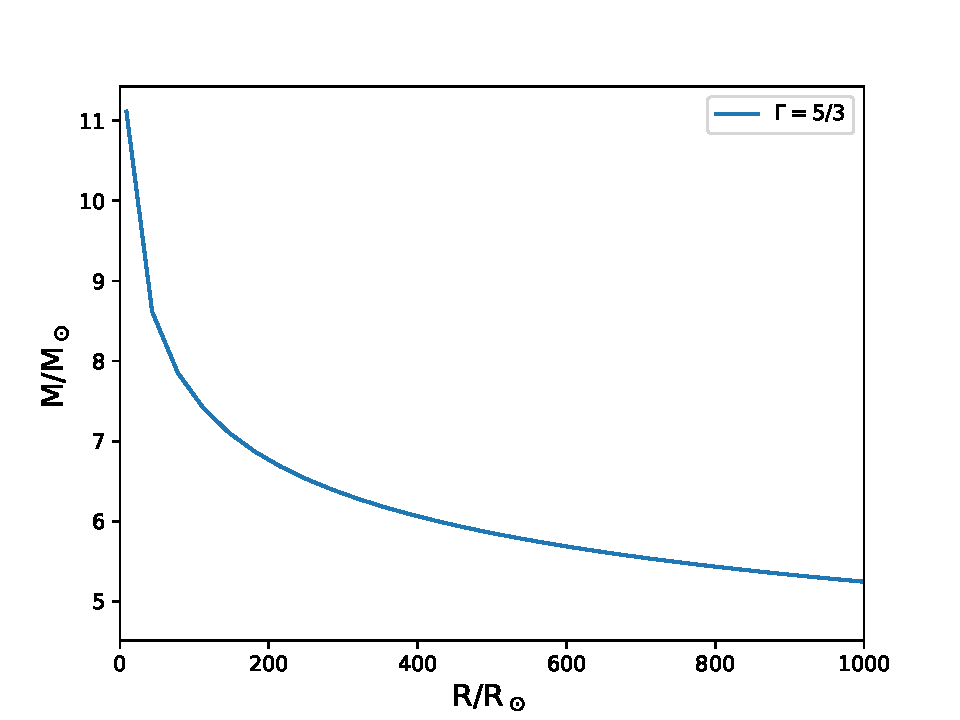
\includegraphics[width=0.7\textwidth, angle=0]{images/polytrope_own.pdf}
\captionsetup{width=.8\textwidth}
\caption{Mass-radius relation for a non-relativistic polytropic star}
\caption*{This mass-radius diagram was computed from equation \ref{M-R}, for a polytropic star with $k=10^{15}$, $\Gamma=5/3$ and a central desity $\rho_0=10^{13}kg/m^3$.}
\label{polytropes1}
\end{center}
\end{figure}

\FloatBarrier

